\documentclass{article}
\usepackage[utf8]{inputenc}
\usepackage[spanish]{babel}
\usepackage{graphicx}
\usepackage{geometry}
\usepackage{enumerate}
\usepackage{titlesec}
\usepackage{float}
\usepackage{listings}
\usepackage{xcolor}
\usepackage{amsmath}
\usepackage{matlab-prettifier}
\usepackage{amssymb}
\usepackage{tabularx}

\geometry{letterpaper, margin = 1.5cm}

\newcommand{\codefontsize}{\fontsize{10}{11}}
\lstset{
	style = Matlab-editor,
	basicstyle = \codefontsize\ttfamily,
	mlshowsectionrules = true,
	upquote = true,
	tabsize = 4,
	captionpos = b,
	breaklines = true,
	breakatwhitespace = true,
	frame = single,
}

%Datos de la Portada
\title{Introducción a la Programación \ Practica 8}
\author{Medina Martinez Jonathan Jason \ 2023640061}
\date{29 de mayo del 2023}

\begin{document}
	
	\fontsize{12}{16}\selectfont
	
	\begin{figure}[t]
		
		
\includegraphics[width=2.5 cm]{Logo1.jpeg}
		\hfill
		
\includegraphics[width=3 cm]{Logo2.png}
		
	\end{figure}
	
	\maketitle
	\newpage
	
	\tableofcontents
	\newpage
	
	\section{Objetivo}
	
	Desarrollo de una interfaz grafica implementando graficas y controles.
	
	\section{Introducción}
	
	El desarrollo de interfaces gráficas es fundamental para crear aplicaciones intuitivas y amigables para los usuarios. En esta práctica, nuestro objetivo es implementar una interfaz gráfica utilizando MATLAB App Designer. La aplicación permitirá al usuario especificar los límites inferiores y superiores de dos vectores, así como el espaciado entre ellos.
	
	\newpage
	\section{Desarrollo}
	
	Utilizando MATLAB App Designer, cree un aplicación que permita especificar al usuario los limites inferiores y superiores para los vectores x y y , así como el espaciamiento de para cada uno de ellos. Use la función \textbf{meshgrid} para mapear $x$ y $y$ en dos nuevas matrices bidimensionales llamadas $X$ y $Y$ . Use sus nuevas matrices para calcular el vector Z, con magnitud:
	
	\begin{equation*}
		Z = \sin (\sqrt{X^2 + Y^2})
	\end{equation*}
	
	El programa deberá mostrar, dentro de la interfaz, las siguientes graficas:
	
	\begin{itemize}
		\item Grafica de malla de $Z$.
		\item Grafica de superficie de $Z$.
		\item Grafica de malla de $Z$ con entradas para las tres dimensiones ($X$, $Y$, $Z$).
		\item Grafica de superficie de $Z$ con entradas para las tres dimensiones ($X$, $Y$, $Z$).
		\item Grafica tridimensional de contorno de $Z$.
		\item Grafica que combine superficie y contorno de $Z$.
	\end{itemize}
	
	\newpage
	
	\subsubsection{app1.mlaap}
	
	\begin{lstlisting}
classdef app1 < matlab.apps.AppBase
	
	% Properties that correspond to app components
	properties (Access = public)
		UIFigure              matlab.ui.Figure
		Graficar              matlab.ui.control.Button
		LimitesuperiorYLabel  matlab.ui.control.Label
		limsY                 matlab.ui.control.Spinner
		LimiteinferiorYLabel  matlab.ui.control.Label
		limiY                 matlab.ui.control.Spinner
		EspaciadoLabel        matlab.ui.control.Label
		Espaciado             matlab.ui.control.Spinner
		LimitesuperiorXLabel  matlab.ui.control.Label
		limsX                 matlab.ui.control.Spinner
		LimiteinferiorXLabel  matlab.ui.control.Label
		limiX                 matlab.ui.control.Spinner
		GraficaSup3D          matlab.ui.control.UIAxes
		GraficaMa3D           matlab.ui.control.UIAxes
		GraficaSupyCon        matlab.ui.control.UIAxes
		GraficaCon            matlab.ui.control.UIAxes
		GraficaSup            matlab.ui.control.UIAxes
		GraficaMa             matlab.ui.control.UIAxes
	end
	
	% Callbacks that handle component events
	methods (Access = private)
	
		% Button pushed function: Graficar
		function GraficarPushed(app, event)
			LimiteInferiorX = app.limiX.Value;
			LimiteSuperiorX = app.limsX.Value;
			
			LimiteInferiorY = app.limiY.Value;
			LimiteSuperiorY = app.limsY.Value;
			
			Espaciamiento = app.Espaciado.Value;
			
			x = LimiteInferiorX:Espaciamiento:LimiteSuperiorX;
			y = LimiteInferiorY:Espaciamiento:LimiteSuperiorY;
			
			[X, Y] = meshgrid(x, y);
			
			Z = sin(sqrt((X.^2) + (Y.^2)));
			
			mesh(app.GraficaMa, X, Z);
			
			surf(app.GraficaSup, X, Z);
			
			mesh(app.GraficaMa3D, X, Y, Z);
			
			surf(app.GraficaSup3D, X, Y, Z);
			
			contour3(app.GraficaCon, X, Y, Z);
			
			surfc(app.GraficaSupyCon, X, Y, Z);
		end
	end
	
	% Component initialization
	methods (Access = private)
	
		% Create UIFigure and components
		function createComponents(app)
		
		% Create UIFigure and hide until all components are created
		app.UIFigure = uifigure('Visible', 'off');
		app.UIFigure.Position = [100 100 981 612];
		app.UIFigure.Name = 'MATLAB App';
		
		% Create GraficaMa
		app.GraficaMa = uiaxes(app.UIFigure);
		title(app.GraficaMa, 'Grafica de Malla')
		xlabel(app.GraficaMa, 'X')
		ylabel(app.GraficaMa, 'Y')
		zlabel(app.GraficaMa, 'Z')
		app.GraficaMa.Position = [420 430 278 178];
		
		% Create GraficaSup
		app.GraficaSup = uiaxes(app.UIFigure);
		title(app.GraficaSup, 'Grafica de Superficie')
		xlabel(app.GraficaSup, 'X')
		ylabel(app.GraficaSup, 'Y')
		zlabel(app.GraficaSup, 'Z')
		app.GraficaSup.Position = [697 430 278 178];
		
		% Create GraficaCon
		app.GraficaCon = uiaxes(app.UIFigure);
		title(app.GraficaCon, 'Grafica 3D de Contorno')
		xlabel(app.GraficaCon, 'X')
		ylabel(app.GraficaCon, 'Y')
		zlabel(app.GraficaCon, 'Z')
		app.GraficaCon.Position = [420 41 278 178];
		
		% Create GraficaSupyCon
		app.GraficaSupyCon = uiaxes(app.UIFigure);
		title(app.GraficaSupyCon, 'Grafica de Superficie y Contorno')
		xlabel(app.GraficaSupyCon, 'X')
		ylabel(app.GraficaSupyCon, 'Y')
		zlabel(app.GraficaSupyCon, 'Z')
		app.GraficaSupyCon.Position = [697 41 278 178];
		
		% Create GraficaMa3D
		app.GraficaMa3D = uiaxes(app.UIFigure);
		title(app.GraficaMa3D, 'Grafica de Malla 3D')
		xlabel(app.GraficaMa3D, 'X')
		ylabel(app.GraficaMa3D, 'Y')
		zlabel(app.GraficaMa3D, 'Z')
		app.GraficaMa3D.Position = [420 234 278 178];
		
		% Create GraficaSup3D
		app.GraficaSup3D = uiaxes(app.UIFigure);
		title(app.GraficaSup3D, 'Grafica de Superficie 3D')
		xlabel(app.GraficaSup3D, 'X')
		ylabel(app.GraficaSup3D, 'Y')
		zlabel(app.GraficaSup3D, 'Z')
		app.GraficaSup3D.Position = [697 234 278 178];
		
		% Create limiX
		app.limiX = uispinner(app.UIFigure);
		app.limiX.Position = [21 542 190 30];
		
		% Create LimiteinferiorXLabel
		app.LimiteinferiorXLabel = uilabel(app.UIFigure);
		app.LimiteinferiorXLabel.Position = [21 571 88 22];
		app.LimiteinferiorXLabel.Text = 'Limite inferior X';
		
		% Create limsX
		app.limsX = uispinner(app.UIFigure);
		app.limsX.Position = [222 542 190 30];
		
		% Create LimitesuperiorXLabel
		app.LimitesuperiorXLabel = uilabel(app.UIFigure);
		app.LimitesuperiorXLabel.Position = [222 571 95 22];
		app.LimitesuperiorXLabel.Text = 'Limite superior X';
		
		% Create Espaciado
		app.Espaciado = uispinner(app.UIFigure);
		app.Espaciado.Step = 0.01;
		app.Espaciado.Limits = [0 Inf];
		app.Espaciado.Position = [23 348 190 30];
		
		% Create EspaciadoLabel
		app.EspaciadoLabel = uilabel(app.UIFigure);
		app.EspaciadoLabel.Position = [23 377 61 22];
		app.EspaciadoLabel.Text = 'Espaciado';
		
		% Create limiY
		app.limiY = uispinner(app.UIFigure);
		app.limiY.Position = [22 443 190 30];
		
		% Create LimiteinferiorYLabel
		app.LimiteinferiorYLabel = uilabel(app.UIFigure);
		app.LimiteinferiorYLabel.Position = [22 472 88 22];
		app.LimiteinferiorYLabel.Text = 'Limite inferior Y';
		
		% Create limsY
		app.limsY = uispinner(app.UIFigure);
		app.limsY.Position = [223 443 190 30];
		
		% Create LimitesuperiorYLabel
		app.LimitesuperiorYLabel = uilabel(app.UIFigure);
		app.LimitesuperiorYLabel.Position = [223 472 95 22];
		app.LimitesuperiorYLabel.Text = 'Limite superior Y';
		
		% Create Graficar
		app.Graficar = uibutton(app.UIFigure, 'push');
		app.Graficar.ButtonPushedFcn = createCallbackFcn(app, @GraficarPushed, true);
		app.Graficar.Position = [109 242 187 30];
		app.Graficar.Text = 'Graficar';
		
		% Show the figure after all components are created
		app.UIFigure.Visible = 'on';
		end
	end
	
	% App creation and deletion
	methods (Access = public)
	
	% Construct app
	function app = app1
	
	% Create UIFigure and components
	createComponents(app)
	
	% Register the app with App Designer
	registerApp(app, app.UIFigure)
	
		if nargout == 0
			clear app
		end
	end
	
	% Code that executes before app deletion
	function delete(app)
	
		% Delete UIFigure when app is deleted
			delete(app.UIFigure)
		end
	end
end
	\end{lstlisting}
	
	\subsubsection{Ejecución}
	
	\begin{figure*}[h]
		\centering
		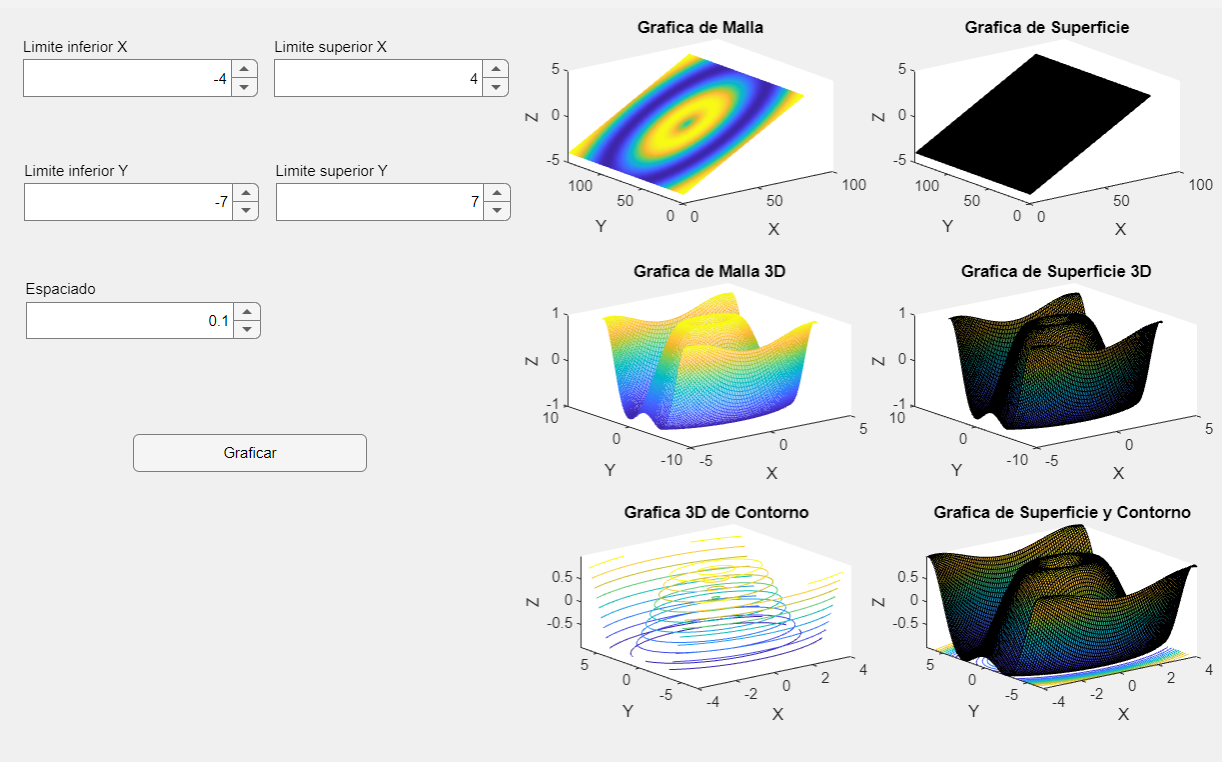
\includegraphics[height = 11 cm]{img1.png}
	\end{figure*}
	
	\newpage
	
	Una vez generadas las graficas, modifique su programa para permitir que el usuario especifique la ecuación que define Z.
	Pruebe su programa con los siguientes datos:
	
	Entrada 1:
	\begin{itemize}
		\item $-4 <= x <= 4$ $espaciamiento: 0.1$
		\item $-7 <= y <= 7$ $espaciamiento: 0.1$
		\item $Z = sin(sqrt(X .^ 2 + Y .^ 2))$
	\end{itemize}
	Entrada 2:
	\begin{itemize}
		\item $0 <= x <= 200$ $espaciamiento: 1$
		\item $0 <= y <= 200$ $espaciamiento: 1$
		\item $Z = membrane(1, 100)$
	\end{itemize}
	
	Entrada 3:
	\begin{itemize}
		\item $-8 <= x <= 8$ $espaciamiento: 0.5$
		\item $-8 <= y <= 8$ $espaciamiento: 0.5$
		\item $Z = sin(sqrt(X .^ 2 + Y .^ 2) + eps)./(sqrt(X .^ 2 + Y .^ 2) + eps)$
	\end{itemize}
	Entrada 4:
	\begin{itemize}
		\item $-5 <= x <= 5$ $espaciamiento: 0.2$
		\item $-5 <= y <= 5$ $espaciamiento: 0.2$
		\item $Z = Y .* \cos(X) - X .* \sin(Y)$
	\end{itemize}
	Entrada 5:
	\begin{itemize}
		\item $-\pi / 2 <= x <= \pi / 2$ $espaciamiento: 0.1$
		\item $-\pi <= y <= \pi$ $espaciamiento: 0.1$
		\item $Z = \cos(X .^ 2 + Y .^ 2) .* (\exp(X .^ 2 - Y .^ 2) + \exp(eps ^ 2 + X .^ 2))$
	\end{itemize}
	
	\newpage
	
	\subsubsection{app2.mlaap}
	
	\begin{lstlisting}
classdef app2 < matlab.apps.AppBase

	% Properties that correspond to app components
	properties (Access = public)
		UIFigure              matlab.ui.Figure
		Formula               matlab.ui.control.EditField
		FormulaLabel          matlab.ui.control.Label
		Graficar              matlab.ui.control.Button
		LimitesuperiorYLabel  matlab.ui.control.Label
		limsY                 matlab.ui.control.Spinner
		LimiteinferiorYLabel  matlab.ui.control.Label
		limiY                 matlab.ui.control.Spinner
		EspaciadoLabel        matlab.ui.control.Label
		Espaciado             matlab.ui.control.Spinner
		LimitesuperiorXLabel  matlab.ui.control.Label
		limsX                 matlab.ui.control.Spinner
		LimiteinferiorXLabel  matlab.ui.control.Label
		limiX                 matlab.ui.control.Spinner
		GraficaSup3D          matlab.ui.control.UIAxes
		GraficaMa3D           matlab.ui.control.UIAxes
		GraficaSupyCon        matlab.ui.control.UIAxes
		GraficaCon            matlab.ui.control.UIAxes
		GraficaSup            matlab.ui.control.UIAxes
		GraficaMa             matlab.ui.control.UIAxes
	end
	
	% Callbacks that handle component events
	methods (Access = private)
		
		% Button pushed function: Graficar
		function GraficarPushed(app, event)
		formula = app.Formula.Value;
		
			LimiteInferiorX = app.limiX.Value;
			LimiteSuperiorX = app.limsX.Value;
			
			LimiteInferiorY = app.limiY.Value;
			LimiteSuperiorY = app.limsY.Value;
			
			Espaciamiento = app.Espaciado.Value;
			
			x = LimiteInferiorX:Espaciamiento:LimiteSuperiorX;
			y = LimiteInferiorY:Espaciamiento:LimiteSuperiorY;
			
			[X, Y] = meshgrid(x, y);
			
			Z = eval(formula);
			
			mesh(app.GraficaMa, X, Z);
			
			surf(app.GraficaSup, X, Z);
			
			mesh(app.GraficaMa3D, X, Y, Z);
			
			surf(app.GraficaSup3D, X, Y, Z);
			
			contour3(app.GraficaCon, X, Y, Z);
			
			surfc(app.GraficaSupyCon, X, Y, Z);
		end
	end
	
	% Component initialization
	methods (Access = private)
	
		% Create UIFigure and components
		function createComponents(app)
		
		% Create UIFigure and hide until all components are created
		app.UIFigure = uifigure('Visible', 'off');
		app.UIFigure.Position = [100 100 981 612];
		app.UIFigure.Name = 'MATLAB App';
		
		% Create GraficaMa
		app.GraficaMa = uiaxes(app.UIFigure);
		title(app.GraficaMa, 'Grafica de Malla')
		xlabel(app.GraficaMa, 'X')
		ylabel(app.GraficaMa, 'Y')
		zlabel(app.GraficaMa, 'Z')
		app.GraficaMa.Position = [420 430 278 178];
		
		% Create GraficaSup
		app.GraficaSup = uiaxes(app.UIFigure);
		title(app.GraficaSup, 'Grafica de Superficie')
		xlabel(app.GraficaSup, 'X')
		ylabel(app.GraficaSup, 'Y')
		zlabel(app.GraficaSup, 'Z')
		app.GraficaSup.Position = [697 430 278 178];
		
		% Create GraficaCon
		app.GraficaCon = uiaxes(app.UIFigure);
		title(app.GraficaCon, 'Grafica 3D de Contorno')
		xlabel(app.GraficaCon, 'X')
		ylabel(app.GraficaCon, 'Y')
		zlabel(app.GraficaCon, 'Z')
		app.GraficaCon.Position = [420 41 278 178];
		
		% Create GraficaSupyCon
		app.GraficaSupyCon = uiaxes(app.UIFigure);
		title(app.GraficaSupyCon, 'Grafica de Superficie y Contorno')
		xlabel(app.GraficaSupyCon, 'X')
		ylabel(app.GraficaSupyCon, 'Y')
		zlabel(app.GraficaSupyCon, 'Z')
		app.GraficaSupyCon.Position = [697 41 278 178];
		
		% Create GraficaMa3D
		app.GraficaMa3D = uiaxes(app.UIFigure);
		title(app.GraficaMa3D, 'Grafica de Malla 3D')
		xlabel(app.GraficaMa3D, 'X')
		ylabel(app.GraficaMa3D, 'Y')
		zlabel(app.GraficaMa3D, 'Z')
		app.GraficaMa3D.Position = [420 234 278 178];
		
		% Create GraficaSup3D
		app.GraficaSup3D = uiaxes(app.UIFigure);
		title(app.GraficaSup3D, 'Grafica de Superficie 3D')
		xlabel(app.GraficaSup3D, 'X')
		ylabel(app.GraficaSup3D, 'Y')
		zlabel(app.GraficaSup3D, 'Z')
		app.GraficaSup3D.Position = [697 234 278 178];
		
		% Create limiX
		app.limiX = uispinner(app.UIFigure);
		app.limiX.Position = [21 542 190 30];
		
		% Create LimiteinferiorXLabel
		app.LimiteinferiorXLabel = uilabel(app.UIFigure);
		app.LimiteinferiorXLabel.Position = [21 571 88 22];
		app.LimiteinferiorXLabel.Text = 'Limite inferior X';
		
		% Create limsX
		app.limsX = uispinner(app.UIFigure);
		app.limsX.Position = [222 542 190 30];
		
		% Create LimitesuperiorXLabel
		app.LimitesuperiorXLabel = uilabel(app.UIFigure);
		app.LimitesuperiorXLabel.Position = [222 571 95 22];
		app.LimitesuperiorXLabel.Text = 'Limite superior X';
		
		% Create Espaciado
		app.Espaciado = uispinner(app.UIFigure);
		app.Espaciado.Step = 0.01;
		app.Espaciado.Limits = [0 Inf];
		app.Espaciado.Position = [23 348 190 30];
		
		% Create EspaciadoLabel
		app.EspaciadoLabel = uilabel(app.UIFigure);
		app.EspaciadoLabel.Position = [23 377 61 22];
		app.EspaciadoLabel.Text = 'Espaciado';
		
		% Create limiY
		app.limiY = uispinner(app.UIFigure);
		app.limiY.Position = [22 443 190 30];
		
		% Create LimiteinferiorYLabel
		app.LimiteinferiorYLabel = uilabel(app.UIFigure);
		app.LimiteinferiorYLabel.Position = [22 472 88 22];
		app.LimiteinferiorYLabel.Text = 'Limite inferior Y';
		
		% Create limsY
		app.limsY = uispinner(app.UIFigure);
		app.limsY.Position = [223 443 190 30];
		
		% Create LimitesuperiorYLabel
		app.LimitesuperiorYLabel = uilabel(app.UIFigure);
		app.LimitesuperiorYLabel.Position = [223 472 95 22];
		app.LimitesuperiorYLabel.Text = 'Limite superior Y';
		
		% Create Graficar
		app.Graficar = uibutton(app.UIFigure, 'push');
		app.Graficar.ButtonPushedFcn = createCallbackFcn(app, @GraficarPushed, true);
		app.Graficar.Position = [109 242 187 30];
		app.Graficar.Text = 'Graficar';
		
		% Create FormulaLabel
		app.FormulaLabel = uilabel(app.UIFigure);
		app.FormulaLabel.Position = [223 377 49 22];
		app.FormulaLabel.Text = 'Formula';
		
		% Create Formula
		app.Formula = uieditfield(app.UIFigure, 'text');
		app.Formula.Position = [223 348 188 30];
		
		% Show the figure after all components are created
		app.UIFigure.Visible = 'on';
		end
	end
	
	% App creation and deletion
	methods (Access = public)
	
		% Construct app
		function app = app2
		
		% Create UIFigure and components
		createComponents(app)
		
		% Register the app with App Designer
		registerApp(app, app.UIFigure)
		
			if nargout == 0
				clear app
			end
		end
		
		% Code that executes before app deletion
		function delete(app)
		
		% Delete UIFigure when app is deleted
		delete(app.UIFigure)
		end
	end
end
	\end{lstlisting}
	
	\newpage
	
	\subsubsection{Ejecución}
	
	Entrada 1
	
	\begin{figure*}[h]
		\centering
		
\includegraphics[width=17cm]{img2.png}
	\end{figure*}
	
	Entrada 2
	
	\begin{figure*}[!h]
		\centering
		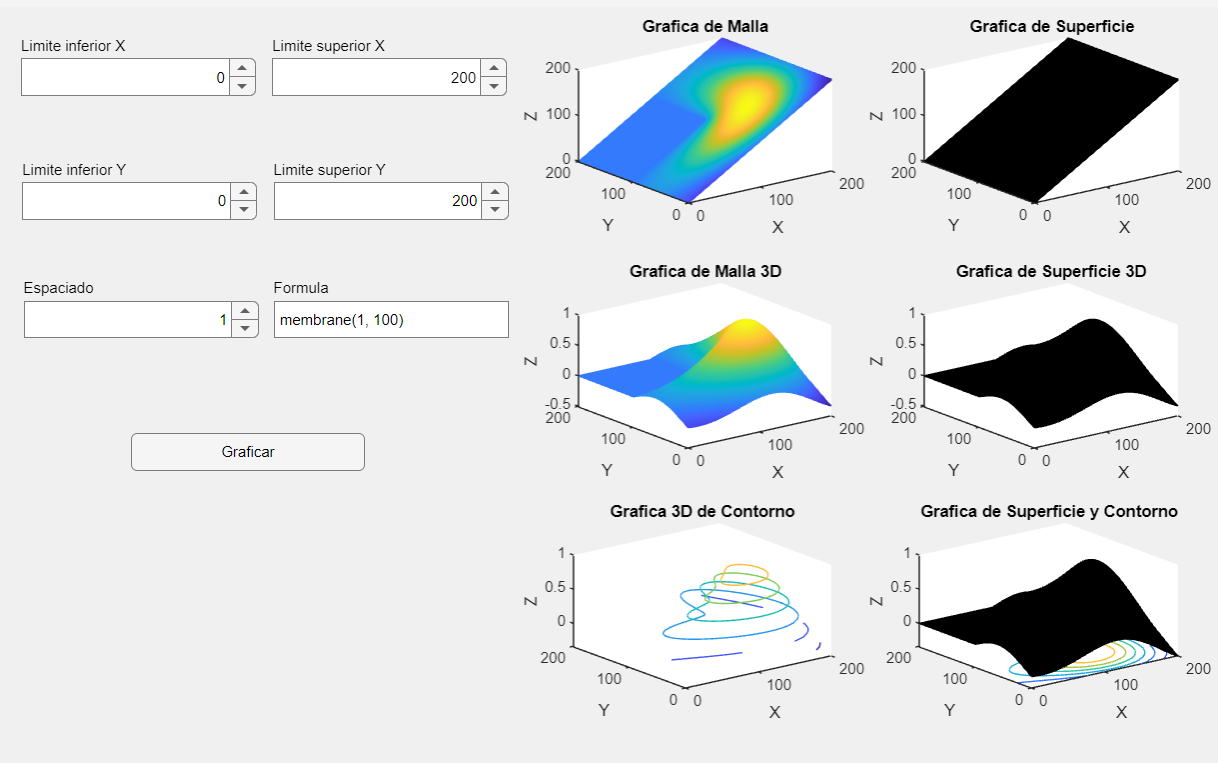
\includegraphics[width=17cm]{img3.png}
	\end{figure*}
	
	\newpage
	
	Entrada 3
	
	\begin{figure*}[h]
		\centering
		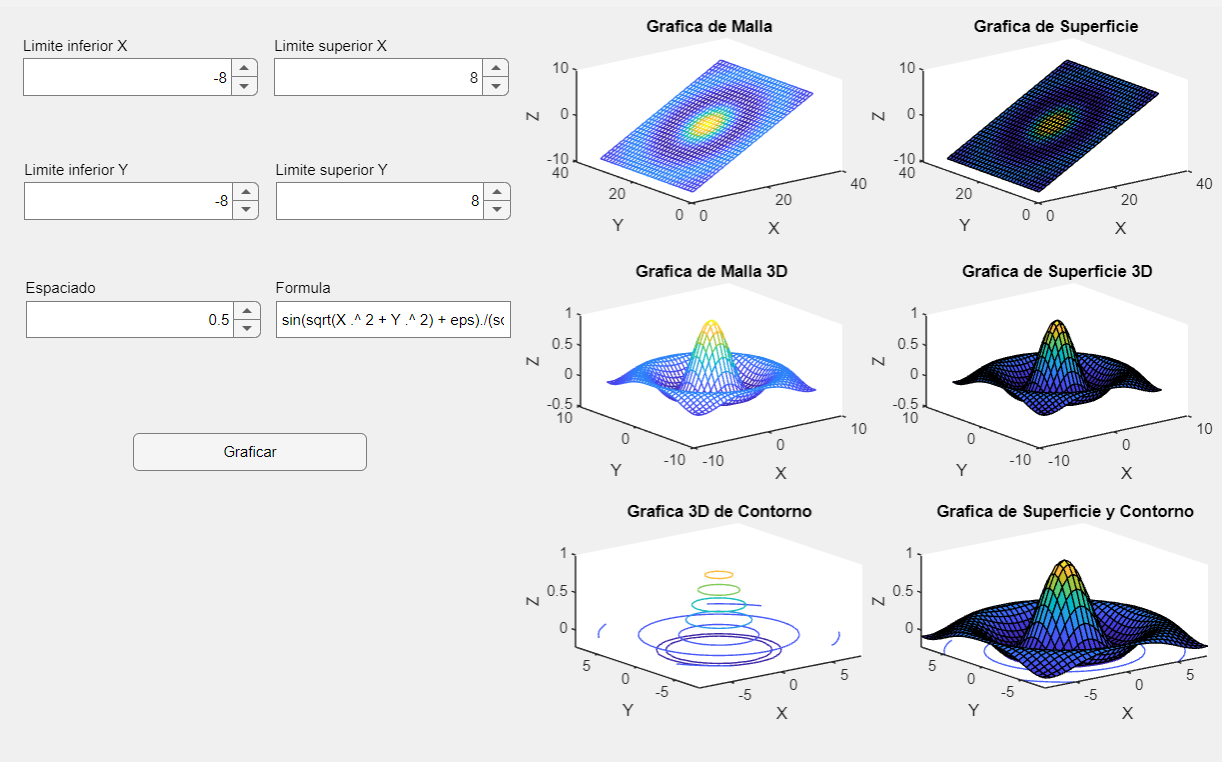
\includegraphics[width=17cm]{img4.png}
	\end{figure*}
	
	Entrada 4
	
	\begin{figure*}[!]
		\centering
		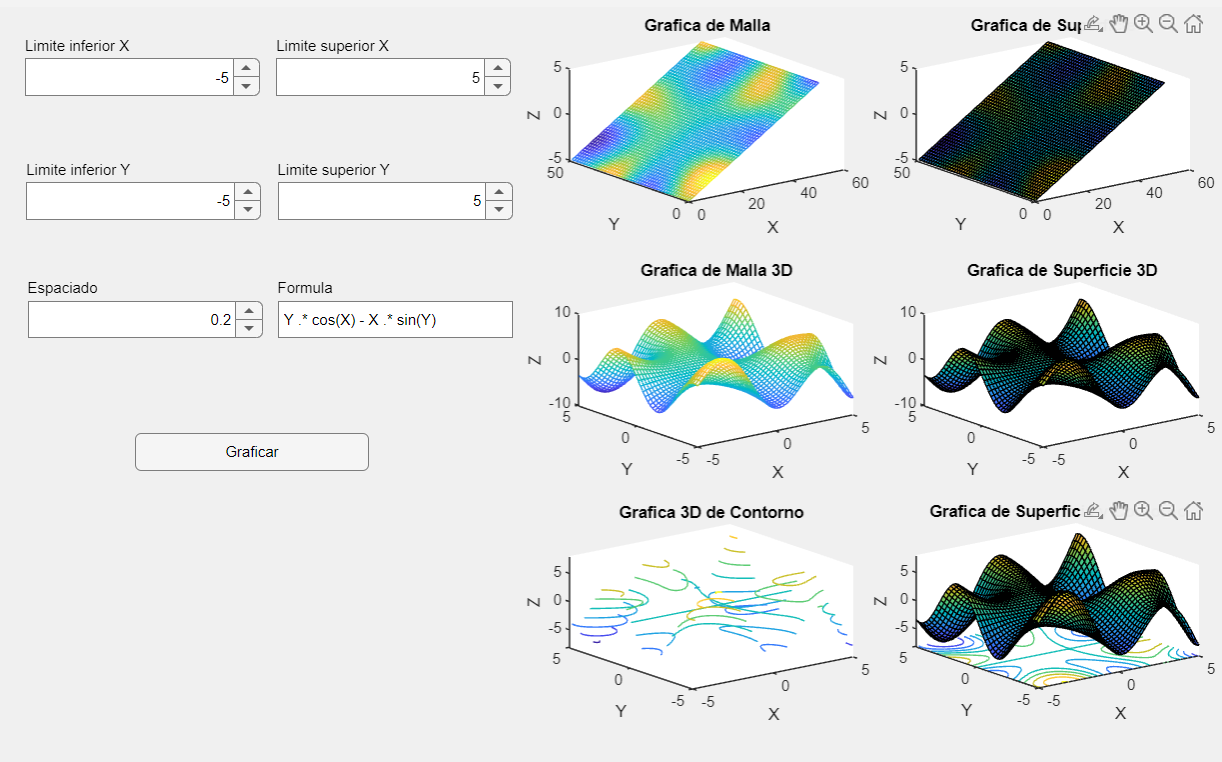
\includegraphics[width=17cm]{img5.png}
	\end{figure*}
	
	\newpage
	
	Entrada 5
	
	\begin{figure*}[h]
		\centering
		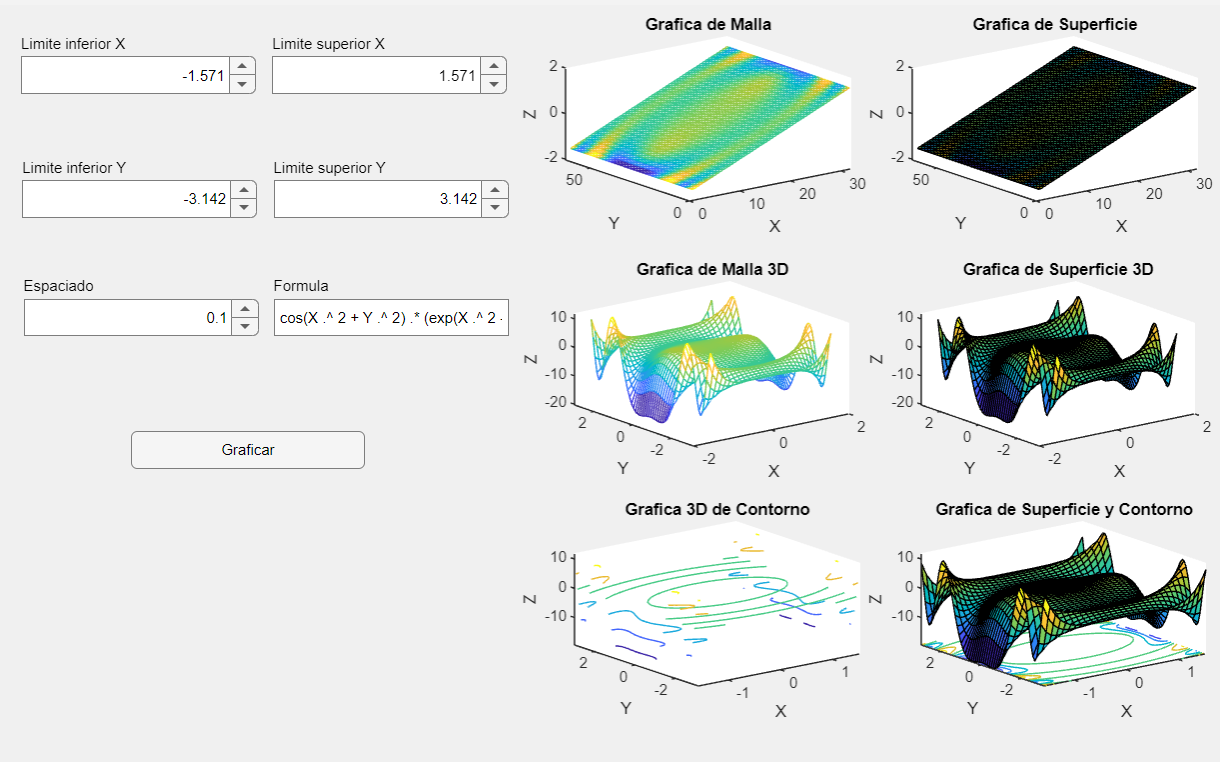
\includegraphics[width=17cm]{img6.png}
	\end{figure*}
	
	\newpage
	
	\section{Conclusión}
	
	En esta práctica, hemos logrado desarrollar una interfaz gráfica utilizando MATLAB App Designer para representar gráficas y controles. A través de la implementación de la función 'meshgrid', pudimos mapear vectores en matrices bidimensionales y calcular el vector 'Z' con base en una ecuación especificada por el usuario. Las gráficas generadas, como las de malla, superficie y contorno de 'Z', proporcionan una representación visual clara de los datos. Además, al permitir que el usuario especifique la ecuación, brindamos flexibilidad y personalización a la aplicación. La prueba con diferentes conjuntos de datos demostró la versatilidad y eficacia de la interfaz gráfica desarrollada. En resumen, esta práctica ha sido exitosa en el desarrollo de una interfaz gráfica interactiva para la visualización de datos utilizando MATLAB.
	
\end{document}